\section{Results}
\label{sec:results}

Every number in this section is read from \texttt{results/*.json} by
\texttt{scripts/paper\_tables.py}, and every figure is drawn from the same files by
\texttt{scripts/make\_figures.py}.

\subsection{Training}

The localizer trained for \TrainFullEpochs{} epochs in \TrainFullMinutes{} minutes on the
\GPU{} (Fig.~\ref{fig:trainloc}). Its best validation epoch was the last one
(\TrainFullBestEpoch), so it had not fully converged. The design history
(Fig.~\ref{fig:history}) shows why the final input and steering layer were needed: both earlier
designs stayed near \AbortOneValMAE$^\circ$ MAE, and the final design without symmetry
augmentation overfit within \NoAugEpochs{} epochs.

PPO ran for \RLSteps{} environment steps in \RLHours{} hours (Fig.~\ref{fig:trainrl}). The mean
episode return rose from \RLFirstReturn{} to about \RLFinalReturn{} (mean of the last 5\% of
updates) and was flat for the last half of training. This is the third attempt. The first
crashed early in training (its log was overwritten, so we do not report its step count), and the
second crashed at \RLCrashTwoSteps{} steps. Both crashes were CUDA errors raised when another GPU
process on the same Windows machine started or exited. The third run
saved a checkpoint every 250{,}000 steps but was not interrupted. The curve of the second run is
kept in \texttt{results/crashed\_rl\_run2\_curve.json}.

The residual network reached a validation duty MAE of \ResValMAE{} over \ResNTrain{} training
samples, against \ResMixerMAE{} for the flat-ground mixer it corrects
(Fig.~\ref{fig:trainres}).

\begin{figure*}[t]
\centering
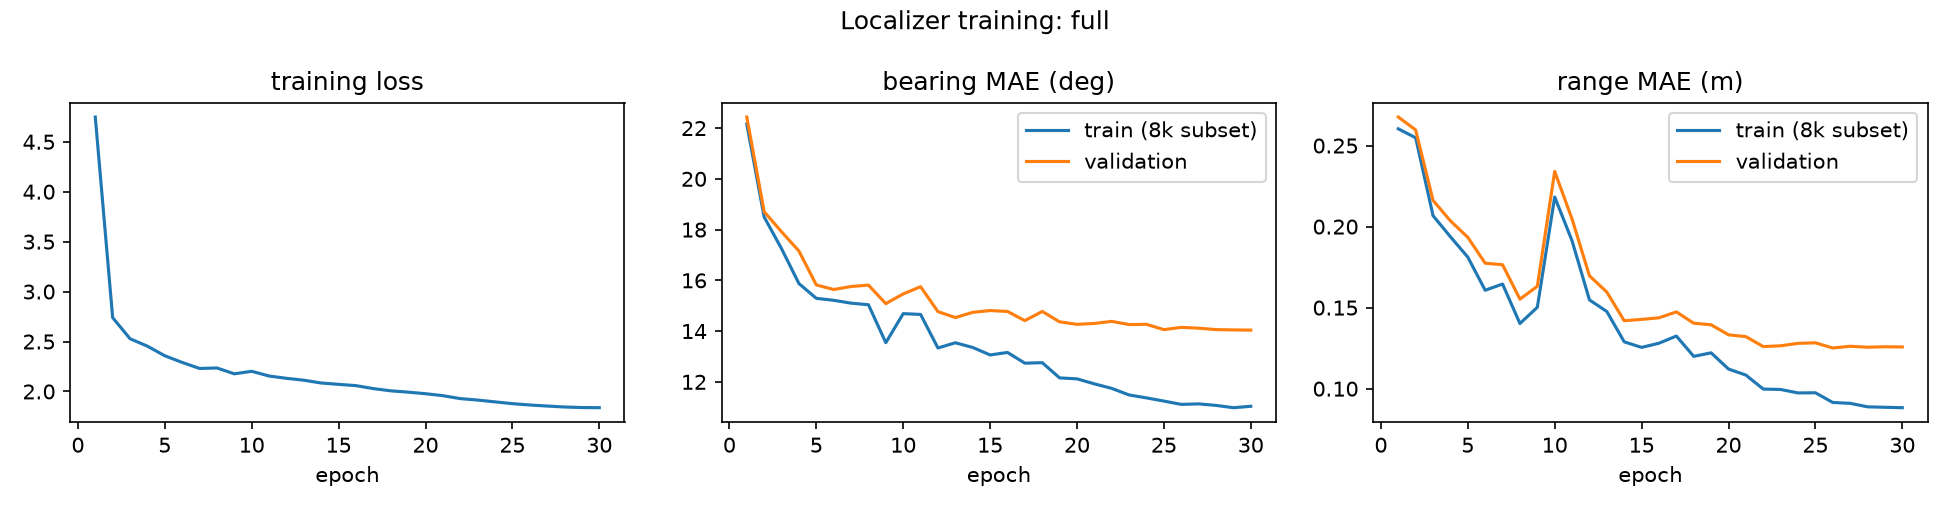
\includegraphics[width=\textwidth]{train_localizer_full.png}
\caption{Localizer training (\TrainFullNTrain{} examples, batch \BatchSize, fp16 on the \GPU).
The training curve is measured on a fixed 8{,}000-example subset with augmentation off.}
\label{fig:trainloc}
\end{figure*}

\begin{figure*}[t]
\centering
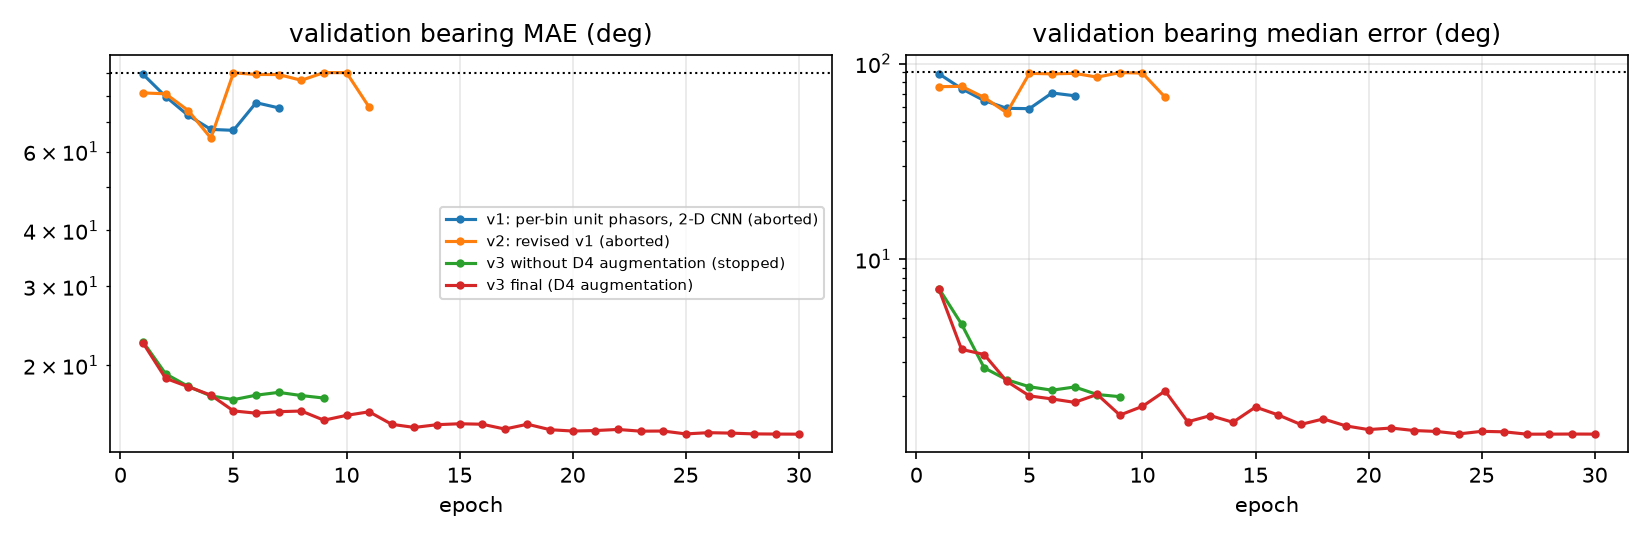
\includegraphics[width=0.85\textwidth]{localizer_design_history.png}
\caption{Validation bearing error of every localizer design we trained, including the two
aborted ones and the stopped run without symmetry augmentation. Dotted line: 90$^\circ$
(chance MAE).}
\label{fig:history}
\end{figure*}

\begin{figure*}[t]
\centering
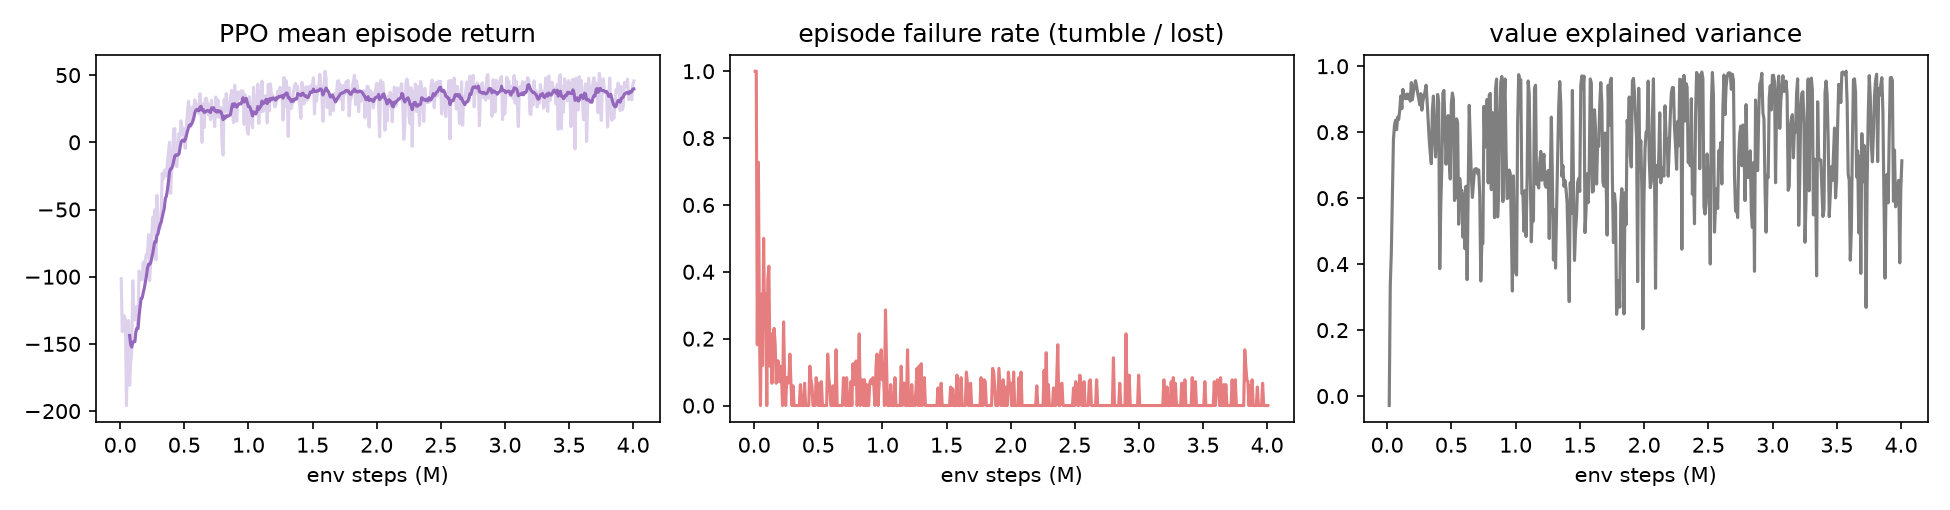
\includegraphics[width=\textwidth]{train_rl.png}
\caption{PPO training, \RLSteps{} steps, \RLEnvs{} parallel environments with random
terrain. Left: mean episode return (light: raw, dark: moving average). Centre: fraction of
episodes ended by a tumble or by losing the person. Right: value-function explained variance.}
\label{fig:trainrl}
\end{figure*}

\begin{figure}[t]
\centering
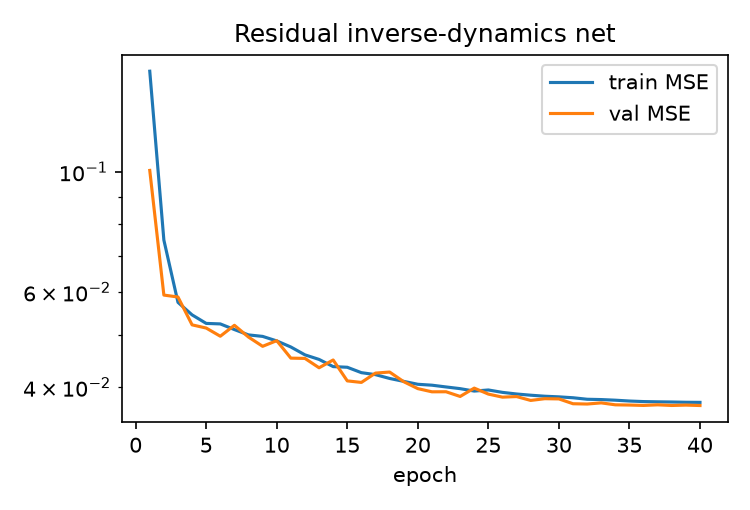
\includegraphics[width=\columnwidth]{train_residual.png}
\caption{Residual inverse-dynamics network, train and validation MSE of the predicted duty.}
\label{fig:trainres}
\end{figure}

\subsection{Localization}

Table~\ref{tab:loc} compares all localizers on the same \NTestSet{} test recordings. The deep
localizer more than halves the classical bearing MAE (\LocdlfullBMAE$^\circ$ against
\LocsrpphatBMAE$^\circ$ for SRP-PHAT and \LocgcclstdoaBMAE$^\circ$ for pairwise GCC-PHAT) and
cuts the median error from \LocsrpphatBMed$^\circ$ to \LocdlfullBMed$^\circ$. Its range MAE
is \LocdlfullRMAE\,m against \LocsrpphatRMAE\,m for matched-filter time of flight. The medians
are close (\LocdlfullRMed{} and \LocsrpphatRMed\,m), so the classical range error comes from a
tail of gross errors where a reflection or noise peak is picked as the first arrival
(Fig.~\ref{fig:loccdf}, right).

The mean bearing error of every method is dominated by low SNR (Fig.~\ref{fig:locsnr}). On the
\SnrAN{} test recordings whose direct-path SNR at the array is below 0\,dB, the deep localizer's
MAE is \LocdlfullSnrABMAE$^\circ$ (SRP-PHAT \LocsrpphatSnrABMAE$^\circ$). From 10 to 20\,dB it is
\LocdlfullSnrCBMAE$^\circ$ (SRP-PHAT \LocsrpphatSnrCBMAE$^\circ$). The mean is therefore a
statement about how often the phone is far, occluded or quiet, more than about the method's
precision.

By front end (Table~\ref{tab:locch}), the ideal channel is easiest (\LocdlfullAusBMAE$^\circ$).
The ultrasonic chirp through the realistic speaker and microphone chain is the hardest
(\LocdlfullBusBMAE$^\circ$, SRP-PHAT \LocsrpphatBusBMAE$^\circ$), because the modelled roll-off
leaves little in-band energy. The 17--19.5\,kHz fallback recovers most of the performance
(\LocdlfullBfbBMAE$^\circ$). By terrain (Table~\ref{tab:locterr}), the deep localizer is best
indoors (\LocdlfullindoorBMAE$^\circ$) and worst on grass (\LocdlfullgrassBMAE$^\circ$), where
ground absorption lowers the SNR. It beats both classical methods on every terrain and channel.

\textbf{Ablations.} Without the phase channels the network is at chance
(\LocdlmagBMAE$^\circ$ MAE, median \LocdlmagBMed$^\circ$), while its range MAE
(\LocdlmagRMAE\,m) is close to that of the full model. This is the expected outcome rather than
a weak baseline. The array's omnidirectional microphones are 10\,cm apart at most, so
level differences between them carry almost no direction, and the inter-channel delays (at most
0.3\,ms, or 14 samples) are invisible in log-power maps with a 32-sample hop. Range survives
because it comes from arrival time. Training without multipath (anechoic training set, normal
test set) raises the bearing MAE from \LocdlfullBMAE$^\circ$ to \LocdlanechoicBMAE$^\circ$ and
the range MAE from \LocdlfullRMAE{} to \LocdlanechoicRMAE\,m. Multipath augmentation helps, but
by less than the input representation does.

\textbf{Latency.} On the \GPU, batched inference costs \LatDlFullBatchedMsPerExample\,ms per
example against \LatClassicalBatchedMsPerExample\,ms for the classical pipeline. A single
example takes \LatDlFullSingleMsGpu\,ms on the GPU and \LatDlFullSingleMsCpu\,ms on the CPU, close
to the 50\,ms chirp period. These timings were taken while a closed-loop evaluation shared the
GPU, so they are upper bounds.

\begin{table*}[t]
\centering
\caption{Localization on the \NTestSet{} test recordings (all terrains and channels).}
\label{tab:loc}
\begin{tabular}{lrrrrrrrr}
\toprule
method & \multicolumn{5}{c}{bearing error (deg)} & \multicolumn{3}{c}{range error (m)}\\
\cmidrule(lr){2-6}\cmidrule(lr){7-9}
 & MAE & RMSE & median & p90 & \% $<10^\circ$ & MAE & RMSE & median\\
\midrule
SRP-PHAT & 23.3 & 45.8 & 5.1 & 80.3 & 55 & 0.69 & 1.77 & 0.09 \\
GCC-PHAT LS-TDOA & 25.2 & 48.6 & 6.1 & 92.0 & 61 & 0.69 & 1.77 & 0.09 \\
DL (mag.+phase) & 13.2 & 34.4 & 1.3 & 38.5 & 78 & 0.12 & 0.32 & 0.06 \\
DL (magnitude only) & 89.3 & 103.1 & 89.0 & 160.9 & 5 & 0.14 & 0.36 & 0.07 \\
DL (no multipath in training) & 15.8 & 37.6 & 2.0 & 46.0 & 73 & 0.15 & 0.35 & 0.08 \\
\bottomrule
\end{tabular}

\end{table*}

\begin{table*}[t]
\centering
\caption{Bearing MAE / median (deg) by front-end channel, same test set.}
\label{tab:locch}
\begin{tabular}{lrrr}
\toprule
method & A\_us & B\_us & B\_fb\\
\midrule
SRP-PHAT & 14.8 / 3.0 & 61.6 / 45.9 & 19.1 / 2.4 \\
GCC-PHAT LS-TDOA & 16.8 / 4.3 & 61.7 / 44.4 & 21.7 / 5.3 \\
DL (mag.+phase) & 6.3 / 1.0 & 44.4 / 19.6 & 9.9 / 1.1 \\
DL (magnitude only) & 88.8 / 88.1 & 91.1 / 91.8 & 89.2 / 89.0 \\
DL (no multipath in training) & 9.2 / 1.6 & 48.4 / 26.2 & 11.3 / 1.5 \\
\bottomrule
\end{tabular}

\end{table*}

\begin{table*}[t]
\centering
\caption{Bearing MAE / median (deg) by terrain, same test set.}
\label{tab:locterr}
\begin{tabular}{lrrrrrr}
\toprule
method & flat & slope & rough & grass & indoor & obstacles\\
\midrule
SRP-PHAT & 20.5 / 2.2 & 24.0 / 7.2 & 22.7 / 5.3 & 28.7 / 9.6 & 20.0 / 6.4 & 23.6 / 3.0 \\
GCC-PHAT LS-TDOA & 23.5 / 5.0 & 26.4 / 7.0 & 24.3 / 5.7 & 29.0 / 6.3 & 22.1 / 6.7 & 26.0 / 5.9 \\
DL (mag.+phase) & 10.7 / 0.8 & 14.4 / 2.0 & 13.5 / 2.0 & 18.4 / 1.3 & 8.3 / 1.0 & 13.9 / 1.0 \\
DL (magnitude only) & 88.8 / 84.2 & 89.0 / 88.3 & 92.9 / 94.3 & 88.8 / 90.9 & 87.5 / 88.5 & 88.7 / 87.2 \\
DL (no multipath in training) & 14.1 / 1.6 & 17.7 / 3.6 & 15.9 / 2.8 & 18.3 / 1.3 & 12.6 / 1.8 & 16.0 / 1.6 \\
\bottomrule
\end{tabular}

\end{table*}

\begin{figure*}[t]
\centering
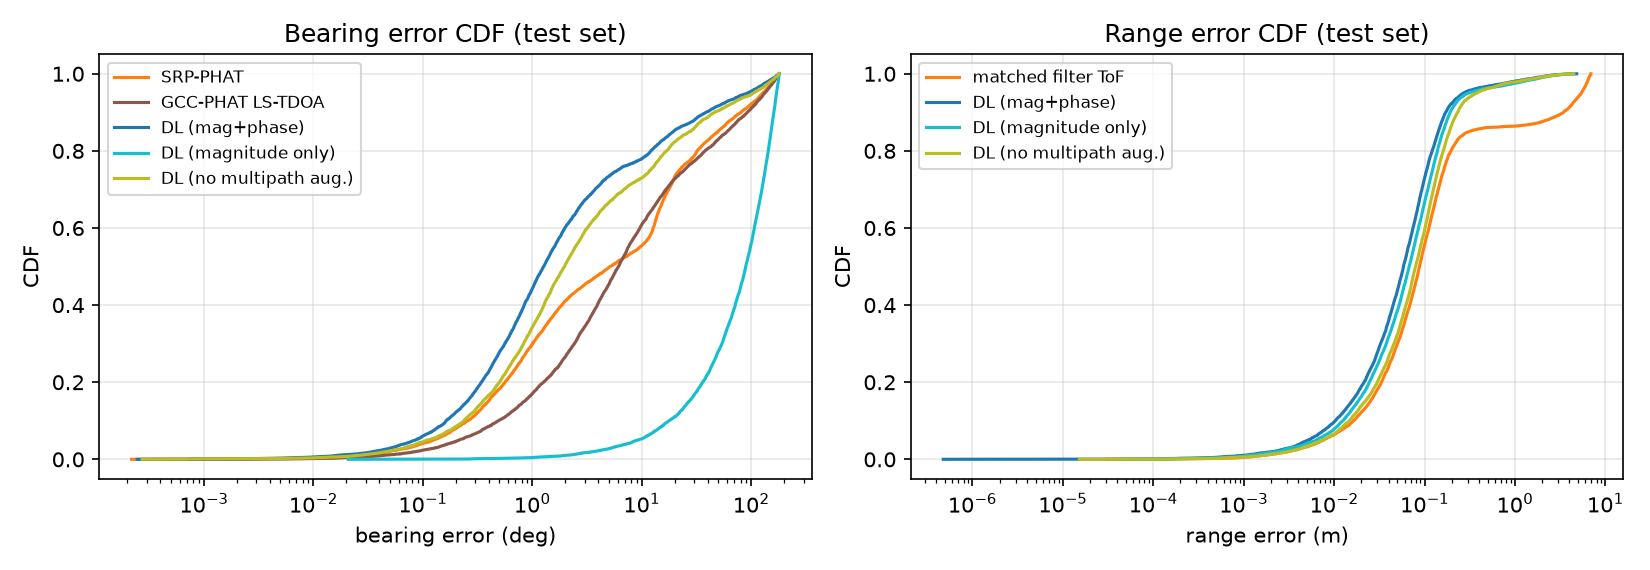
\includegraphics[width=\textwidth]{loc_cdf.png}
\caption{Error CDFs on the test set. Range for SRP-PHAT is the matched-filter time of flight.}
\label{fig:loccdf}
\end{figure*}

\begin{figure*}[t]
\centering
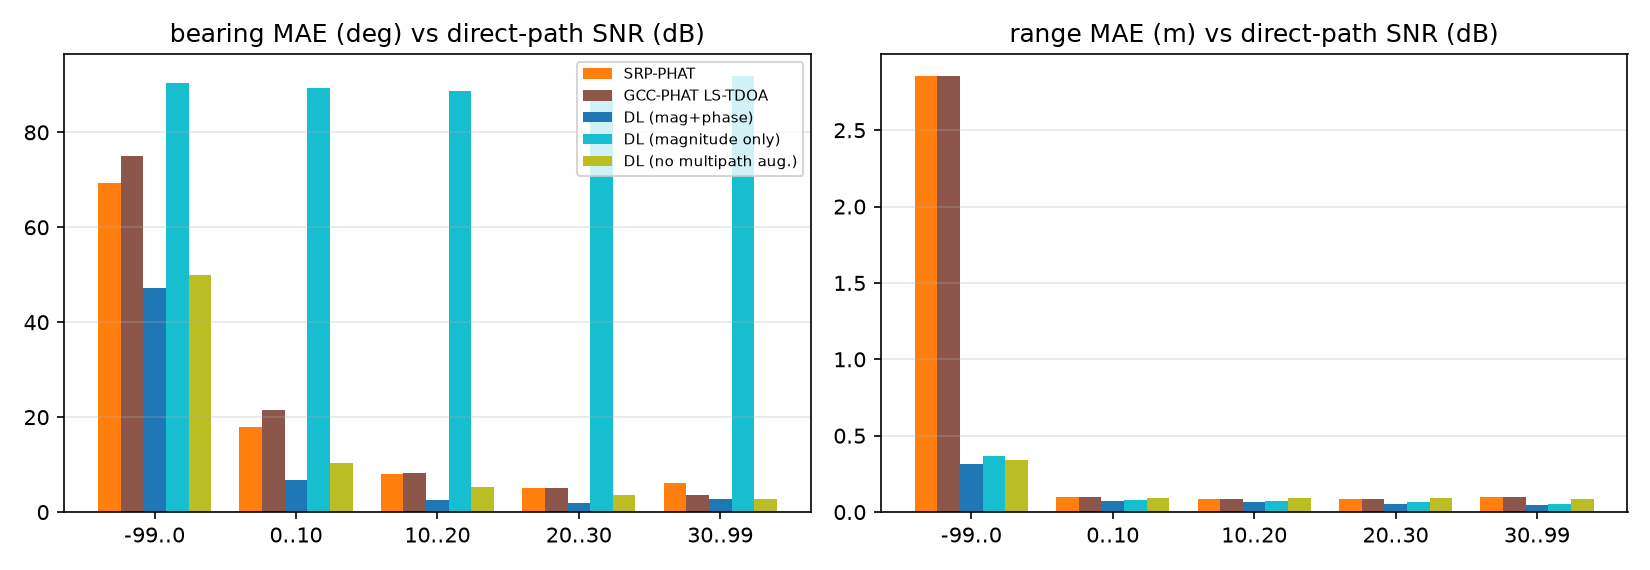
\includegraphics[width=\textwidth]{loc_vs_snr.png}
\caption{Bearing and range MAE by direct-path SNR at the array.}
\label{fig:locsnr}
\end{figure*}

\begin{figure*}[t]
\centering
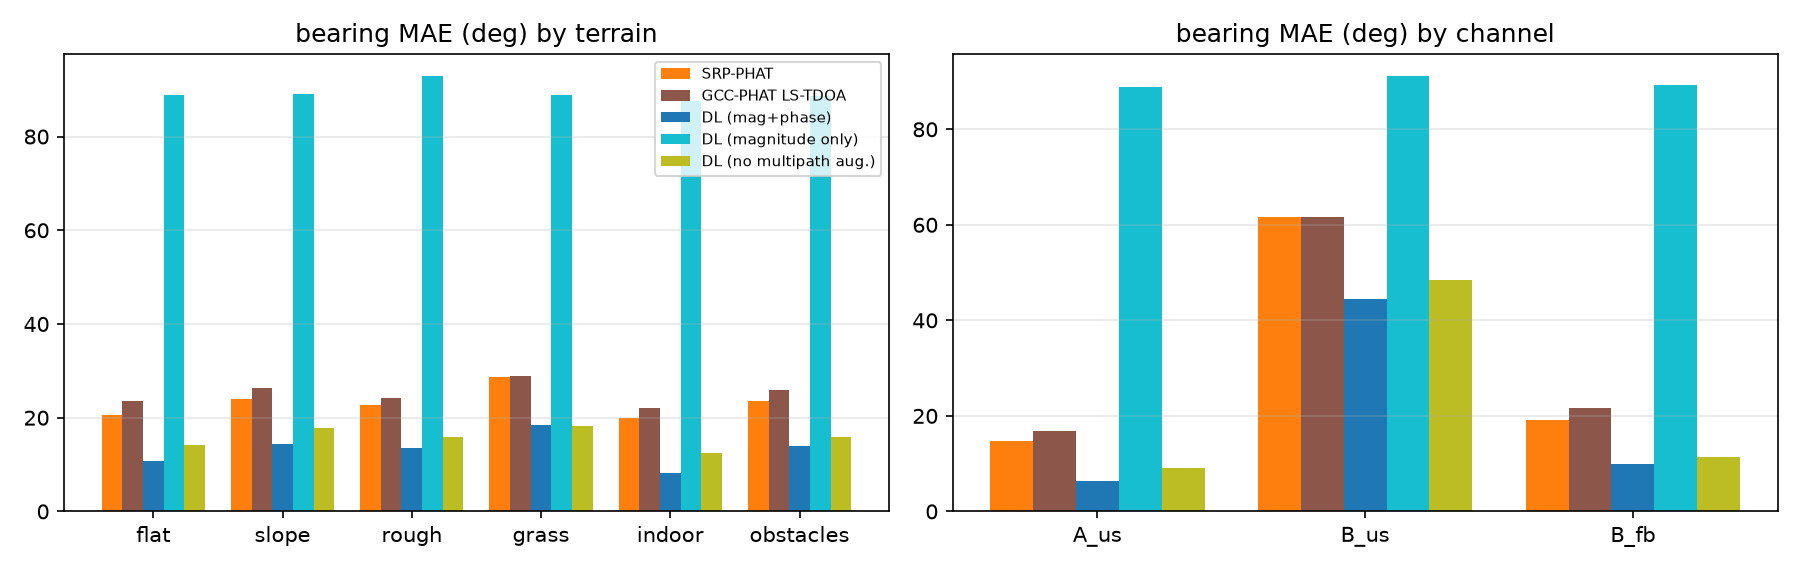
\includegraphics[width=\textwidth]{loc_by_terrain_channel.png}
\caption{Bearing MAE by terrain and by front-end channel.}
\label{fig:locterr}
\end{figure*}

\subsection{Closed-loop following, ideal channel}

Tables~\ref{tab:clsucc}--\ref{tab:clextra} and Fig.~\ref{fig:clbars} give the closed-loop
results on channel A\_us, with \CLAusN{} episodes of \CLAusSeconds\,s per terrain and the
same scenarios for every controller.

\textbf{Localization quality carries through to following where the vehicle is easy to
drive.} On flat, rough, indoor and obstacle terrain, the oracle succeeds in every episode and
the tracker-based controllers come close. The deep localizer keeps the robot nearer to the
person than GCC-PHAT does: pooled mean distance is \CLAusdltrackdist\,m against
\CLAusgcctrackdist\,m, and final distance \CLAusdltrackfinal{} against \CLAusgcctrackfinal\,m. In
closed loop the in-the-loop bearing error is \CLAusdltrackbmae$^\circ$ against
\CLAusgcctrackbmae$^\circ$ (Table~\ref{tab:clbmae}). It is lower than the test-set errors
because the robot keeps the person close and in front.

\textbf{Where the vehicle is hard to drive, control dominates.} On slope and grass even the
oracle succeeds in only \CLAusoraclesuccslope\% and \CLAusoraclesuccgrass\% of episodes, so the
pursuit law, not the localizer, is the bottleneck. The PPO policy is the only controller that
handles slopes (\CLAusrlsuccslope\% success against \CLAusoraclesuccslope\% for the oracle and
\CLAusdltracksuccslope\% for DL + tracker). It is also the best on grass
(\CLAusrlsuccgrass\%), and it does this with the classical acoustic features only. Its pooled
success rate is the highest of all methods (\CLAusrlsucc\% against \CLAusoraclesucc\% for the
oracle). Its control effort (\CLAusrleffort) is close to the oracle's (\CLAusoracleeffort),
and it spends the least time closer than 0.4\,m (\CLAusrlclose\%). On flat ground it trails slightly behind
(\CLAusrldistflat\,m mean distance against \CLAusdltrackdistflat\,m for DL + tracker), as if it
had learned a looser standoff.

\textbf{DL + PID tumbles, and the residual fixes it.} The cascaded PID holds the standoff
tightly on easy terrain, with mean distance \CLAusdlpiddistflat\,m on flat ground. But it
tumbles: \CLAusdlpidtumbles{} tumble steps per episode pooled, and \CLAusdlpidtumblesindoor{}
indoors, where only \CLAusdlpidsuccindoor\% of episodes succeed. With oracle localization
(\DbgN{} scenarios, \DbgSeconds\,s, \texttt{results/debug\_pid\_indoor.json}) it does not
tumble indoors, but its peak cart pitch reaches \DbgOraclePidindoorPitch\,rad against the
\PitchLimit\,rad limit, against \DbgOraclePursuitindoorPitch\,rad for the pursuit law. Its
duty is saturated \DbgOraclePidindoorSat\% of the time. The inner speed loop
reacts to every stop and start of the person with full duty, and small localization errors over
a 60\,s episode push the cart past the limit. Our PID has no pitch limiter; a practical one
would need it.

Adding the residual raises success indoors to \CLAusdlpidressuccindoor\%, on flat ground to
\CLAusdlpidressuccflat\% and pooled to \CLAusdlpidressucc\% (from \CLAusdlpidsucc\%), and it
cuts tumbles to \CLAusdlpidrestumbles{} per episode. The mechanism is visible with oracle
localization. The residual raises the mean duty but lowers the peak pitch, indoors from
\DbgOraclePidindoorPitch{} to \DbgOraclePidResindoorPitch\,rad and on flat ground from
\DbgOraclePidflatPitch{} to \DbgOraclePidResflatPitch\,rad. Because the feedforward already
supplies the duty the terrain needs, the integrator does less of the work and overshoots less.
The cost is the highest control effort of all methods (\CLAusdlpidreseffort). On slopes neither
PID variant works (\CLAusdlpidsuccslope\% and \CLAusdlpidressuccslope\%). On grass both beat the
pursuit law (\CLAusdlpidsuccgrass\% against \CLAusdltracksuccgrass\% for DL + tracker), because
their integrators make up for the higher rolling resistance.

\textbf{Grass is limited by sensing at range as well.} On grass every controller except the
oracle falls behind late in the episodes (Fig.~\ref{fig:cldist}). Ground absorption lowers the
SNR as the distance grows, the localizer degrades, and the robot loses ground. The DL bearing
error in the loop is \CLAusdltrackbmaegrass$^\circ$ on grass against
\CLAusdltrackbmaeflat$^\circ$ on flat ground.

\begin{table*}[t]
\centering
\caption{Follow success rate (\%), channel A\_us, \CLAusN{} episodes per terrain. Success:
within \FollowRadius\,m of the person for at least \SuccessFrac\% of the time after a \WarmupS\,s
warm-up, and no tumble.}
\label{tab:clsucc}
\begin{tabular}{lrrrrrrr}
\toprule
method & flat & slope & rough & grass & indoor & obstacles & all\\
\midrule
Oracle + pursuit & 100 & 50 & 100 & 30 & 100 & 100 & 80 \\
GCC-PHAT + tracker & 97 & 17 & 93 & 17 & 100 & 97 & 70 \\
DL + tracker & 97 & 37 & 100 & 20 & 100 & 93 & 74 \\
DL + PID & 80 & 13 & 87 & 47 & 23 & 87 & 56 \\
DL + PID + residual & 100 & 17 & 93 & 47 & 97 & 100 & 76 \\
RL (PPO) & 93 & 93 & 97 & 63 & 100 & 97 & 91 \\
\bottomrule
\end{tabular}

\end{table*}

\begin{table*}[t]
\centering
\caption{Mean distance to the person after warm-up (m), channel A\_us. The standoff is
\Standoff\,m.}
\label{tab:cldist}
\begin{tabular}{lrrrrrrr}
\toprule
method & flat & slope & rough & grass & indoor & obstacles & all\\
\midrule
Oracle + pursuit & 0.85 & 1.34 & 0.94 & 1.51 & 0.80 & 0.86 & 1.05 \\
GCC-PHAT + tracker & 1.29 & 3.95 & 1.34 & 2.27 & 0.88 & 1.09 & 1.80 \\
DL + tracker & 1.20 & 2.01 & 0.95 & 1.84 & 0.82 & 0.97 & 1.30 \\
DL + PID & 0.84 & 4.58 & 0.86 & 1.51 & 0.81 & 0.84 & 1.57 \\
DL + PID + residual & 0.82 & 4.26 & 0.85 & 1.54 & 0.80 & 0.82 & 1.52 \\
RL (PPO) & 1.39 & 2.15 & 1.22 & 1.92 & 0.80 & 1.01 & 1.41 \\
\bottomrule
\end{tabular}

\end{table*}

\begin{table*}[t]
\centering
\caption{Control effort, mean $u^2$ over both wheels, channel A\_us.}
\label{tab:cleffort}
\begin{tabular}{lrrrrrrr}
\toprule
method & flat & slope & rough & grass & indoor & obstacles & all\\
\midrule
Oracle + pursuit & 0.197 & 0.425 & 0.262 & 0.499 & 0.189 & 0.208 & 0.297 \\
GCC-PHAT + tracker & 0.225 & 0.546 & 0.281 & 0.475 & 0.206 & 0.239 & 0.329 \\
DL + tracker & 0.211 & 0.505 & 0.273 & 0.504 & 0.190 & 0.221 & 0.317 \\
DL + PID & 0.328 & 0.669 & 0.365 & 0.603 & 0.295 & 0.335 & 0.433 \\
DL + PID + residual & 0.428 & 0.718 & 0.466 & 0.670 & 0.390 & 0.435 & 0.518 \\
RL (PPO) & 0.216 & 0.377 & 0.281 & 0.521 & 0.200 & 0.230 & 0.304 \\
\bottomrule
\end{tabular}

\end{table*}

\begin{table*}[t]
\centering
\caption{Bearing error of the localizer in the loop (deg), channel A\_us. RL has no explicit
bearing estimate.}
\label{tab:clbmae}
\begin{tabular}{lrrrrrrr}
\toprule
method & flat & slope & rough & grass & indoor & obstacles & all\\
\midrule
Oracle + pursuit & 0.0 & 0.0 & 0.0 & 0.0 & 0.0 & 0.0 & 0.0 \\
GCC-PHAT + tracker & 10.0 & 12.9 & 10.0 & 14.3 & 7.7 & 9.1 & 10.7 \\
DL + tracker & 4.3 & 4.1 & 1.6 & 7.4 & 1.7 & 3.8 & 3.8 \\
DL + PID & 1.5 & 6.0 & 2.5 & 7.2 & 2.2 & 1.6 & 3.5 \\
DL + PID + residual & 1.4 & 10.2 & 2.2 & 7.4 & 1.8 & 1.5 & 4.1 \\
RL (PPO) & -- & -- & -- & -- & -- & -- & -- \\
\bottomrule
\end{tabular}

\end{table*}

\begin{table*}[t]
\centering
\caption{Further metrics, channel A\_us, pooled over all terrains and episodes.}
\label{tab:clextra}
\begin{tabular}{lrrrrrrrr}
\toprule
method & \% time within & final dist. & time to reach & path & person path & collision & tumbles & \% time\\
 & radius & (m) & radius (s) & (m) & (m) & steps & /episode & $<0.4$ m\\
\midrule
Oracle + pursuit & 90 & 1.05 & 3.9 & 29.4 & 27.3 & 2.0 & 0.00 & 1.5 \\
GCC-PHAT + tracker & 80 & 2.87 & 4.7 & 32.7 & 27.3 & 2.3 & 0.04 & 1.7 \\
DL + tracker & 85 & 1.55 & 4.2 & 30.8 & 27.3 & 3.0 & 0.17 & 1.6 \\
DL + PID & 86 & 2.74 & 4.1 & 35.6 & 27.3 & 2.1 & 2.51 & 1.3 \\
DL + PID + residual & 84 & 2.58 & 4.2 & 35.0 & 27.3 & 1.9 & 0.03 & 1.3 \\
RL (PPO) & 93 & 1.90 & 3.8 & 28.1 & 27.3 & 2.7 & 0.00 & 0.7 \\
\bottomrule
\end{tabular}

\end{table*}

\begin{figure*}[t]
\centering
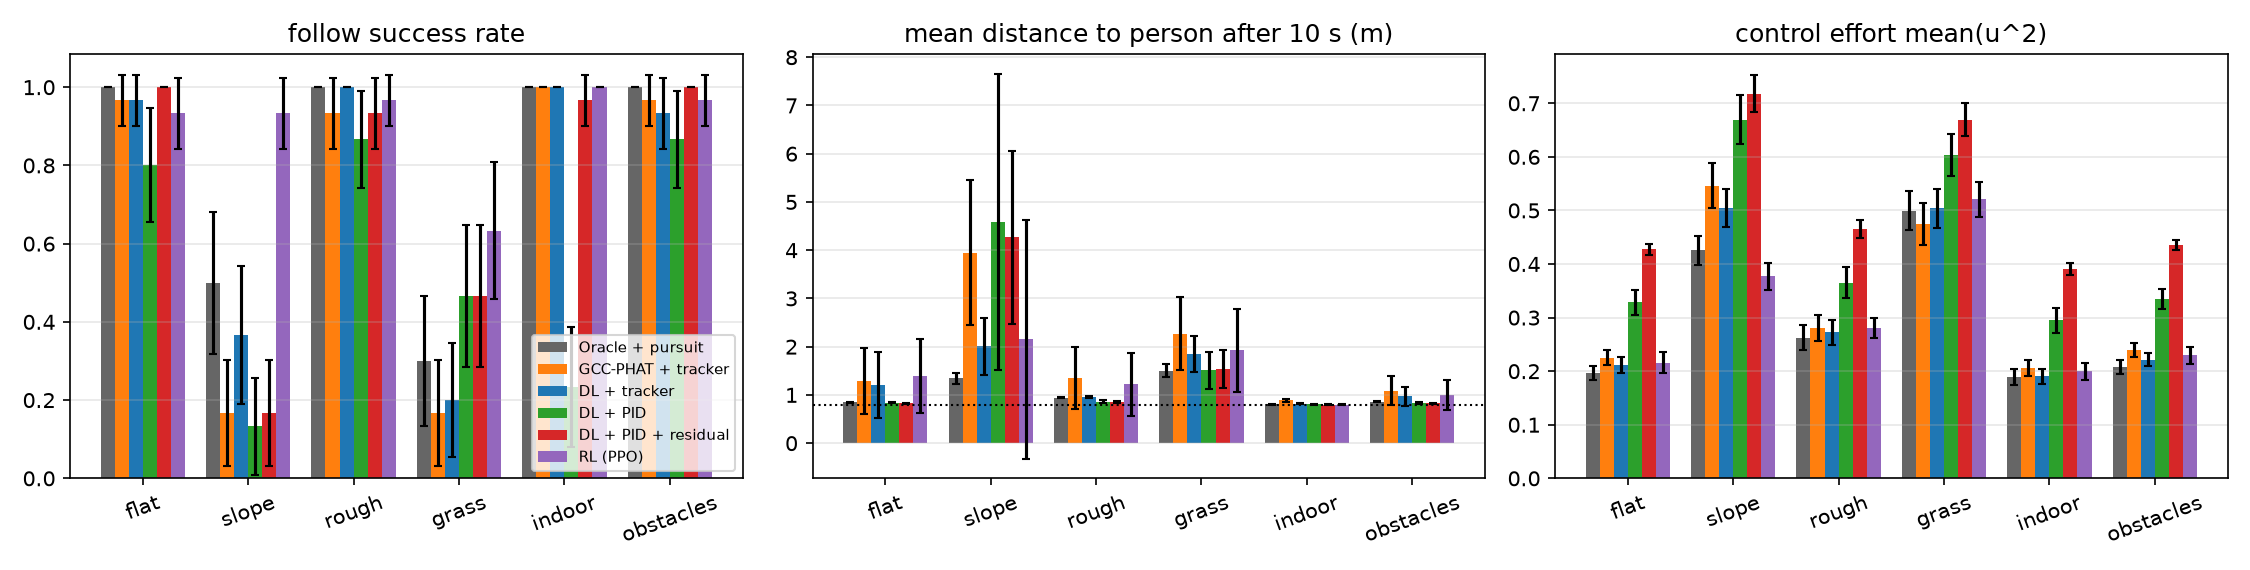
\includegraphics[width=\textwidth]{closed_loop_bars_A_us.png}
\caption{Closed-loop results on channel A\_us. Error bars: 95\% intervals over \CLAusN{} episodes.}
\label{fig:clbars}
\end{figure*}

\begin{figure*}[t]
\centering
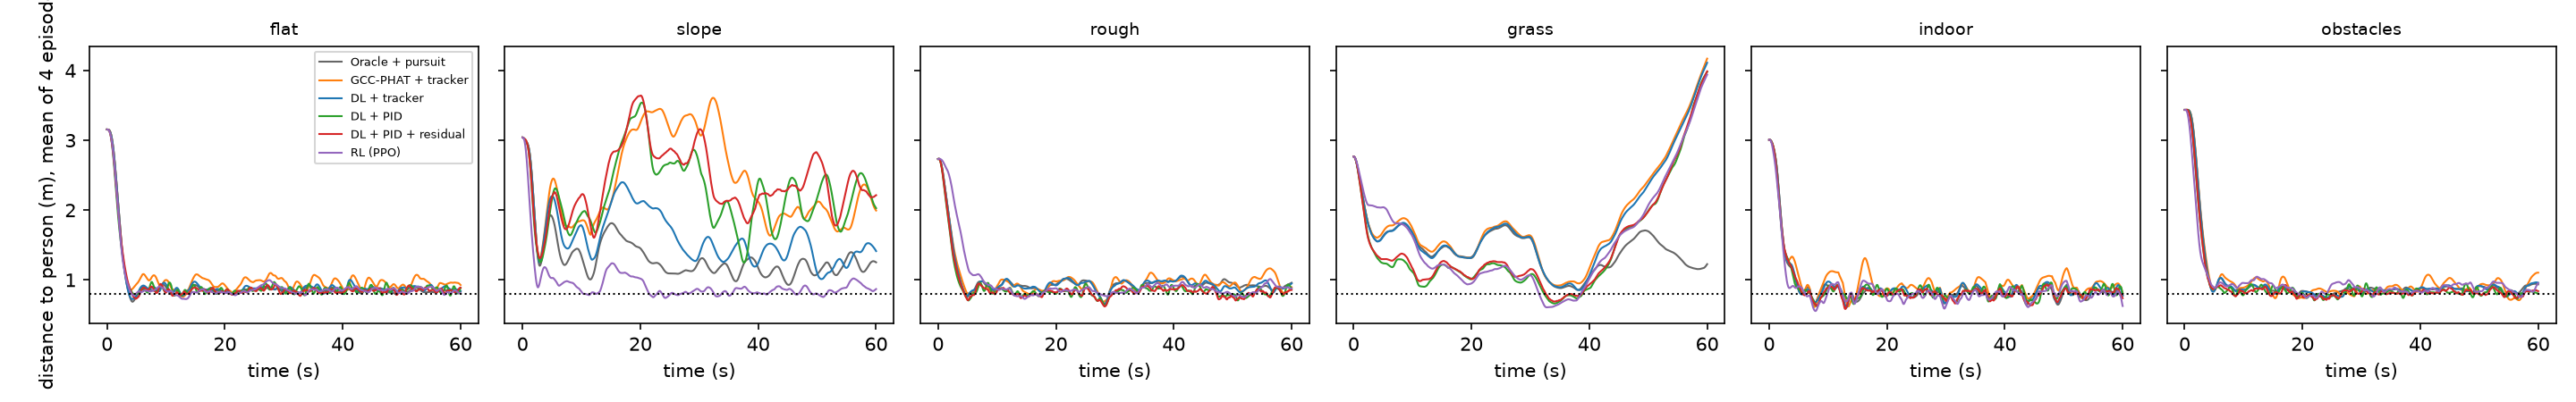
\includegraphics[width=\textwidth]{distance_curves_A_us.png}
\caption{Distance to the person over time, mean of the first four episodes per terrain,
channel A\_us. Dotted: standoff.}
\label{fig:cldist}
\end{figure*}

\begin{figure*}[t]
\centering
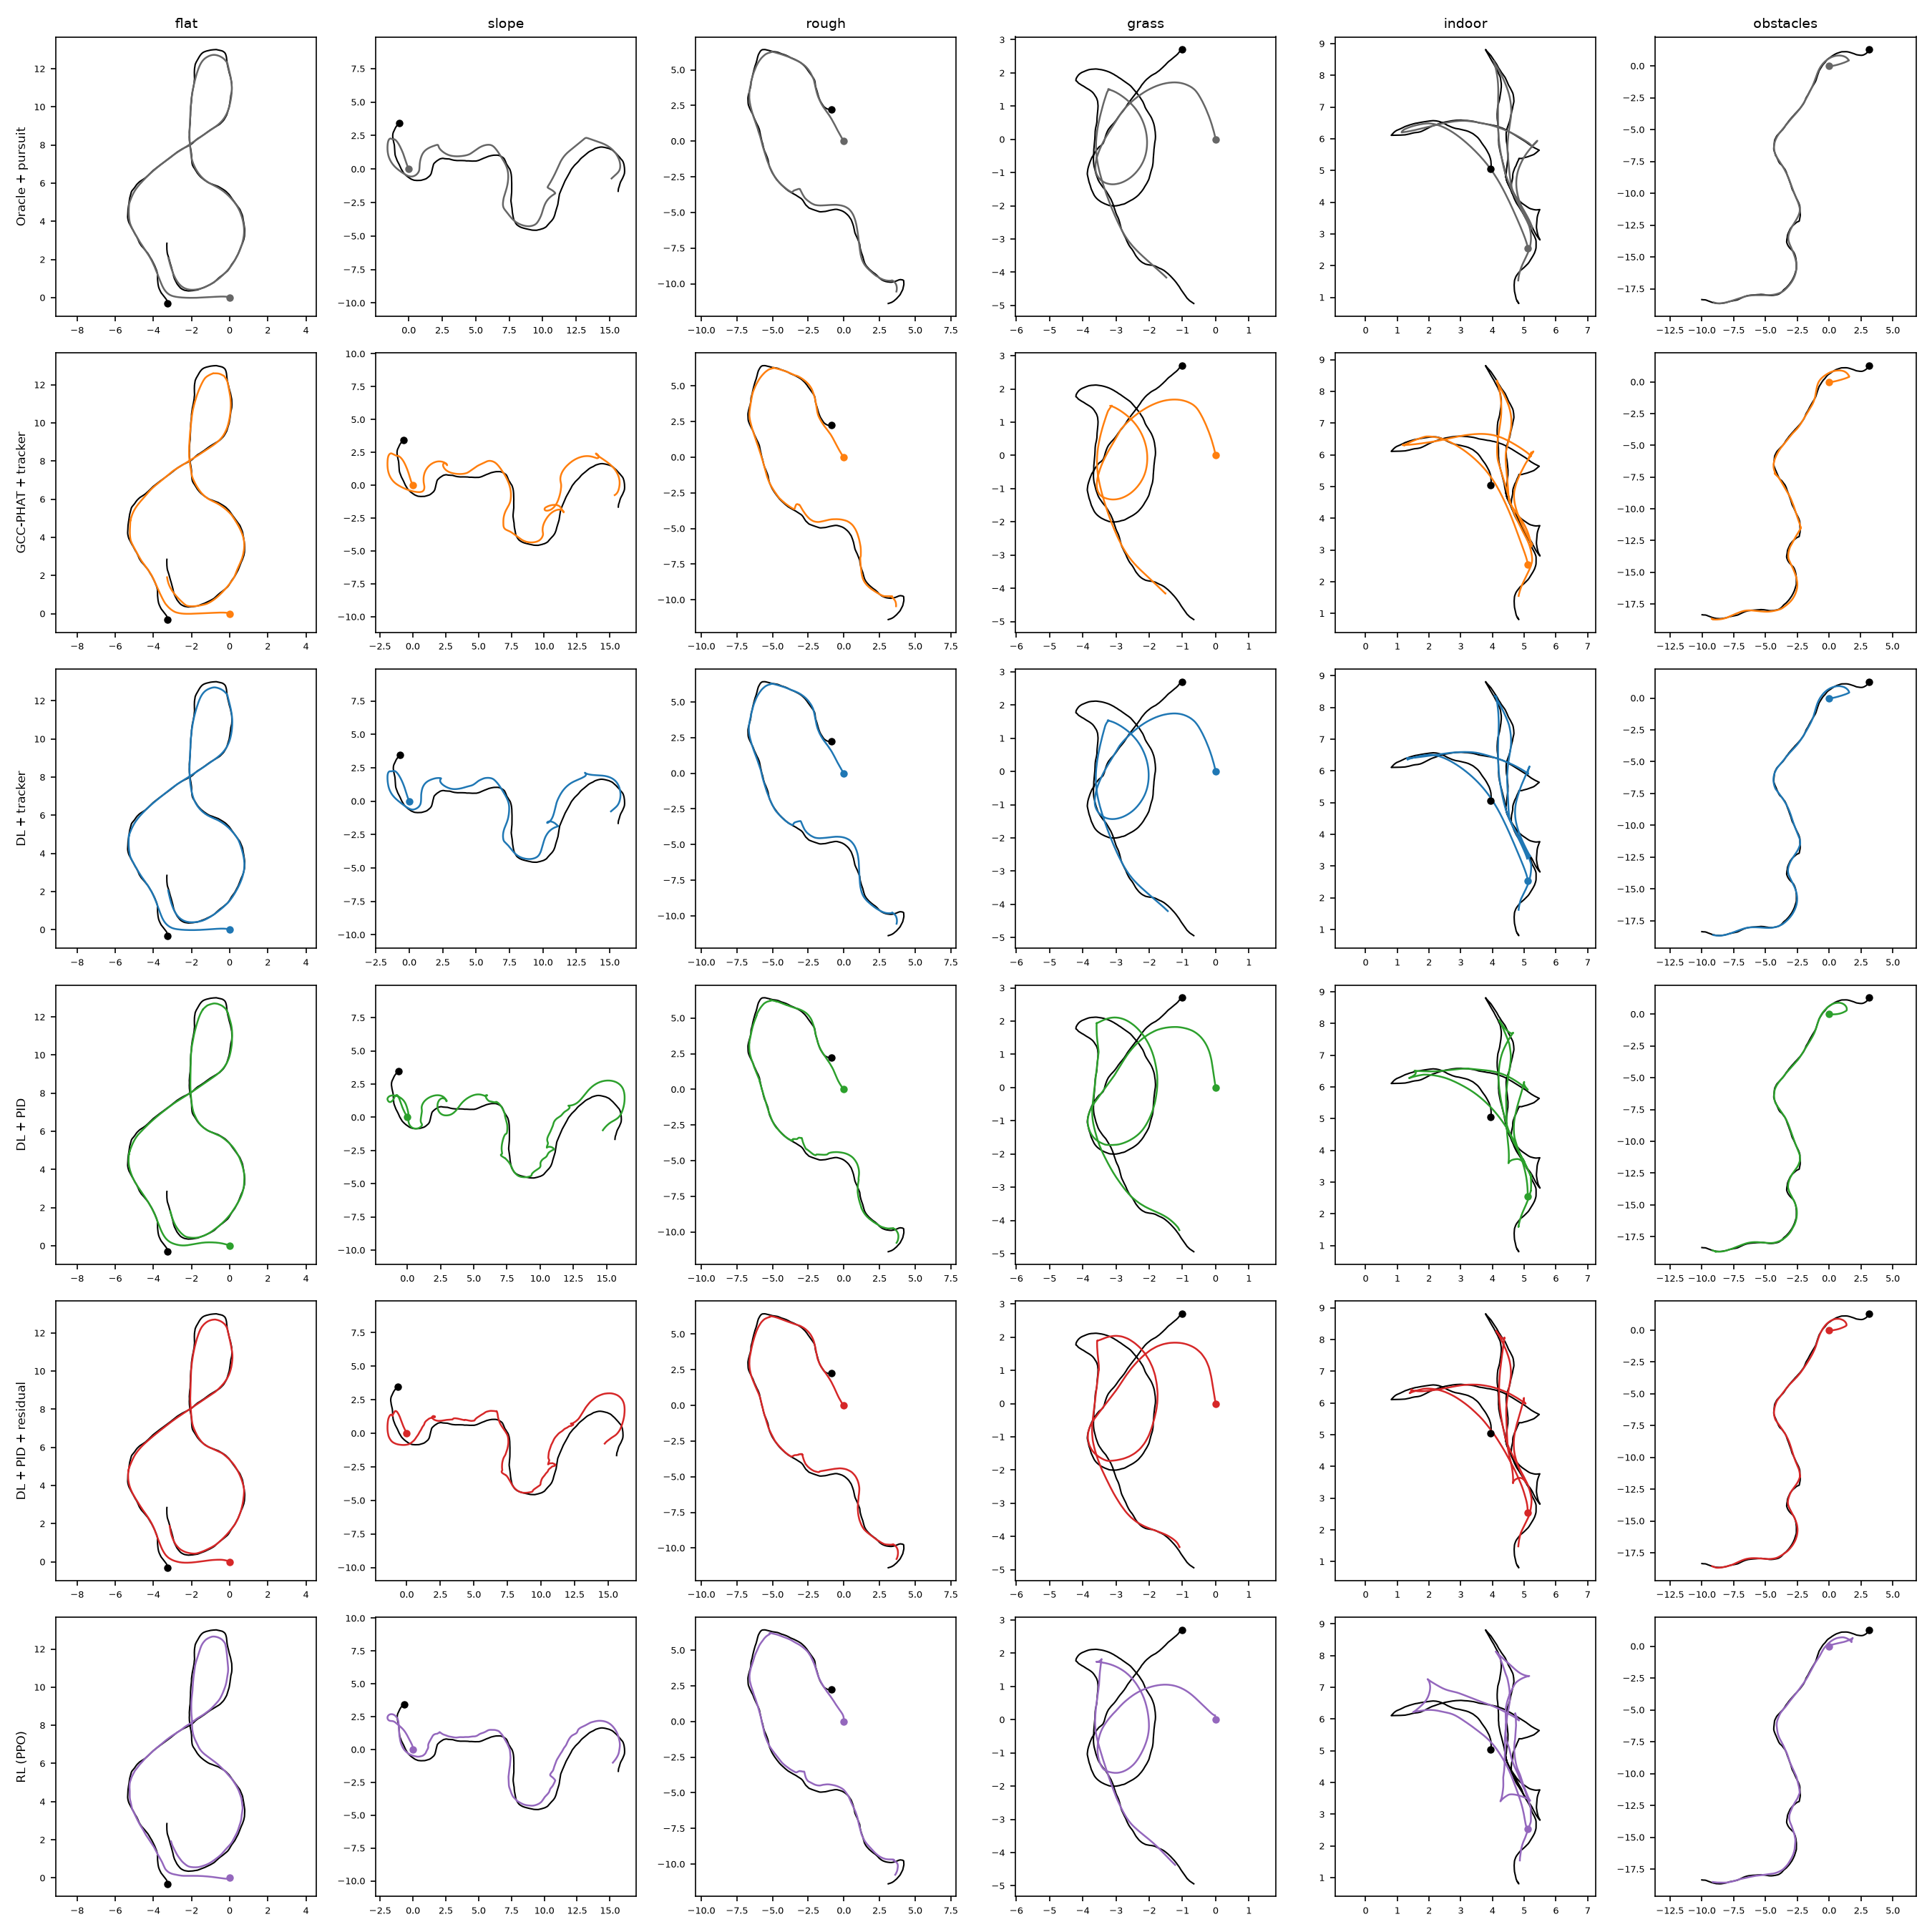
\includegraphics[width=\textwidth]{trajectories_A_us.png}
\caption{First-episode trajectories per controller (rows) and terrain (columns), channel
A\_us. Black: person; colour: robot; dots: start.}
\label{fig:cltraj}
\end{figure*}

\begin{figure}[t]
\centering
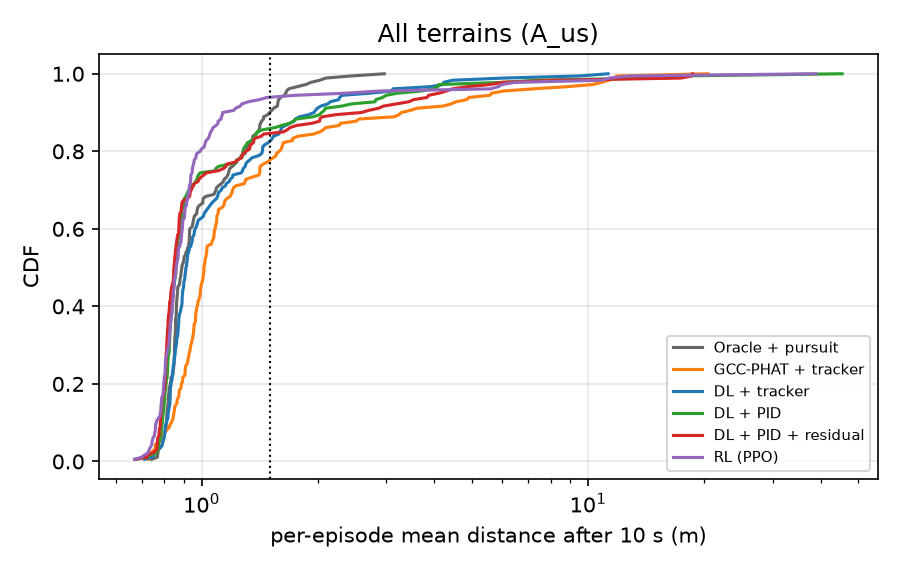
\includegraphics[width=\columnwidth]{closed_loop_cdf_A_us.png}
\caption{CDF of the per-episode mean distance, all terrains, channel A\_us. Dotted: follow
radius.}
\label{fig:clcdf}
\end{figure}

\subsection{Closed-loop following, realistic channel with fallback chirp}

Table~\ref{tab:bfbsucc} repeats the evaluation on channel B\_fb (realistic front end, 17--19.5\,kHz
chirp) with the same scenarios. The deep localizer was trained on all three channels. The RL
policy was trained only on A\_us, so B\_fb is out of distribution for it.

The realistic front end widens the gap between the localizers. In the loop, GCC-PHAT's bearing
error rises to \CLBfbgcctrackbmae$^\circ$ (from \CLAusgcctrackbmae$^\circ$ on A\_us), while the
deep localizer's rises only to \CLBfbdltrackbmae$^\circ$ (from \CLAusdltrackbmae$^\circ$). DL +
tracker keeps its success rate (\CLBfbdltracksucc\% pooled, \CLAusdltracksucc\% on A\_us) and
GCC-PHAT + tracker drops to \CLBfbgcctracksucc\%, with a final distance of
\CLBfbgcctrackfinal\,m against \CLBfbdltrackfinal\,m. DL + PID + residual reaches
\CLBfbdlpidressucc\%. It is again far more reliable than DL + PID (\CLBfbdlpidsucc\%,
\CLBfbdlpidtumbles{} tumble steps per episode against \CLBfbdlpidrestumbles). PPO, out of
distribution, falls from \CLAusrlsucc\% to \CLBfbrlsucc\%. It is still the best controller on
slopes (\CLBfbrlsuccslope\%) and grass (\CLBfbrlsuccgrass\%), but it is no longer the best on
flat ground (\CLBfbrlsuccflat\% against \CLBfbdltracksuccflat\% for DL + tracker), and its
final distance (\CLBfbrlfinal\,m) is the second largest after GCC-PHAT. With realistic
hardware, a policy trained on the features of one front end loses part of its advantage, and
better sensing becomes more valuable.

\begin{table*}[t]
\centering
\caption{Follow success rate (\%), channel B\_fb, \CLBfbN{} episodes per terrain.}
\label{tab:bfbsucc}
\begin{tabular}{lrrrrrrr}
\toprule
method & flat & slope & rough & grass & indoor & obstacles & all\\
\midrule
Oracle + pursuit & 100 & 50 & 100 & 30 & 100 & 100 & 80 \\
GCC-PHAT + tracker & 83 & 20 & 83 & 17 & 97 & 90 & 65 \\
DL + tracker & 97 & 37 & 100 & 23 & 100 & 100 & 76 \\
DL + PID & 60 & 13 & 77 & 47 & 30 & 87 & 52 \\
DL + PID + residual & 100 & 20 & 97 & 50 & 100 & 97 & 77 \\
RL (PPO) & 80 & 77 & 87 & 57 & 97 & 87 & 81 \\
\bottomrule
\end{tabular}

\end{table*}

\begin{table*}[t]
\centering
\caption{Mean distance after warm-up (m), channel B\_fb.}
\label{tab:bfbdist}
\begin{tabular}{lrrrrrrr}
\toprule
method & flat & slope & rough & grass & indoor & obstacles & all\\
\midrule
Oracle + pursuit & 0.85 & 1.34 & 0.94 & 1.51 & 0.80 & 0.86 & 1.05 \\
GCC-PHAT + tracker & 2.01 & 7.72 & 1.61 & 3.09 & 0.94 & 1.65 & 2.84 \\
DL + tracker & 1.21 & 2.23 & 0.95 & 2.29 & 0.82 & 0.87 & 1.40 \\
DL + PID & 1.19 & 5.63 & 0.86 & 1.57 & 0.81 & 0.84 & 1.82 \\
DL + PID + residual & 0.83 & 3.85 & 0.85 & 1.52 & 0.80 & 0.83 & 1.45 \\
RL (PPO) & 2.20 & 5.39 & 2.01 & 2.59 & 0.86 & 1.79 & 2.47 \\
\bottomrule
\end{tabular}

\end{table*}

\begin{table*}[t]
\centering
\caption{Further metrics, channel B\_fb, pooled over all terrains and episodes.}
\label{tab:bfbextra}
\begin{tabular}{lrrrrrrrr}
\toprule
method & \% time within & final dist. & time to reach & path & person path & collision & tumbles & \% time\\
 & radius & (m) & radius (s) & (m) & (m) & steps & /episode & $<0.4$ m\\
\midrule
Oracle + pursuit & 90 & 1.05 & 3.9 & 29.4 & 27.3 & 2.0 & 0.00 & 1.5 \\
GCC-PHAT + tracker & 74 & 4.49 & 5.2 & 31.7 & 27.3 & 2.0 & 0.07 & 1.7 \\
DL + tracker & 85 & 1.93 & 4.5 & 31.1 & 27.3 & 2.9 & 0.00 & 1.6 \\
DL + PID & 85 & 3.18 & 4.2 & 36.0 & 27.3 & 2.6 & 2.57 & 1.2 \\
DL + PID + residual & 85 & 2.03 & 4.0 & 34.6 & 27.3 & 1.8 & 0.07 & 1.4 \\
RL (PPO) & 85 & 3.67 & 4.3 & 29.1 & 27.3 & 3.8 & 0.00 & 0.7 \\
\bottomrule
\end{tabular}

\end{table*}

\begin{figure*}[t]
\centering
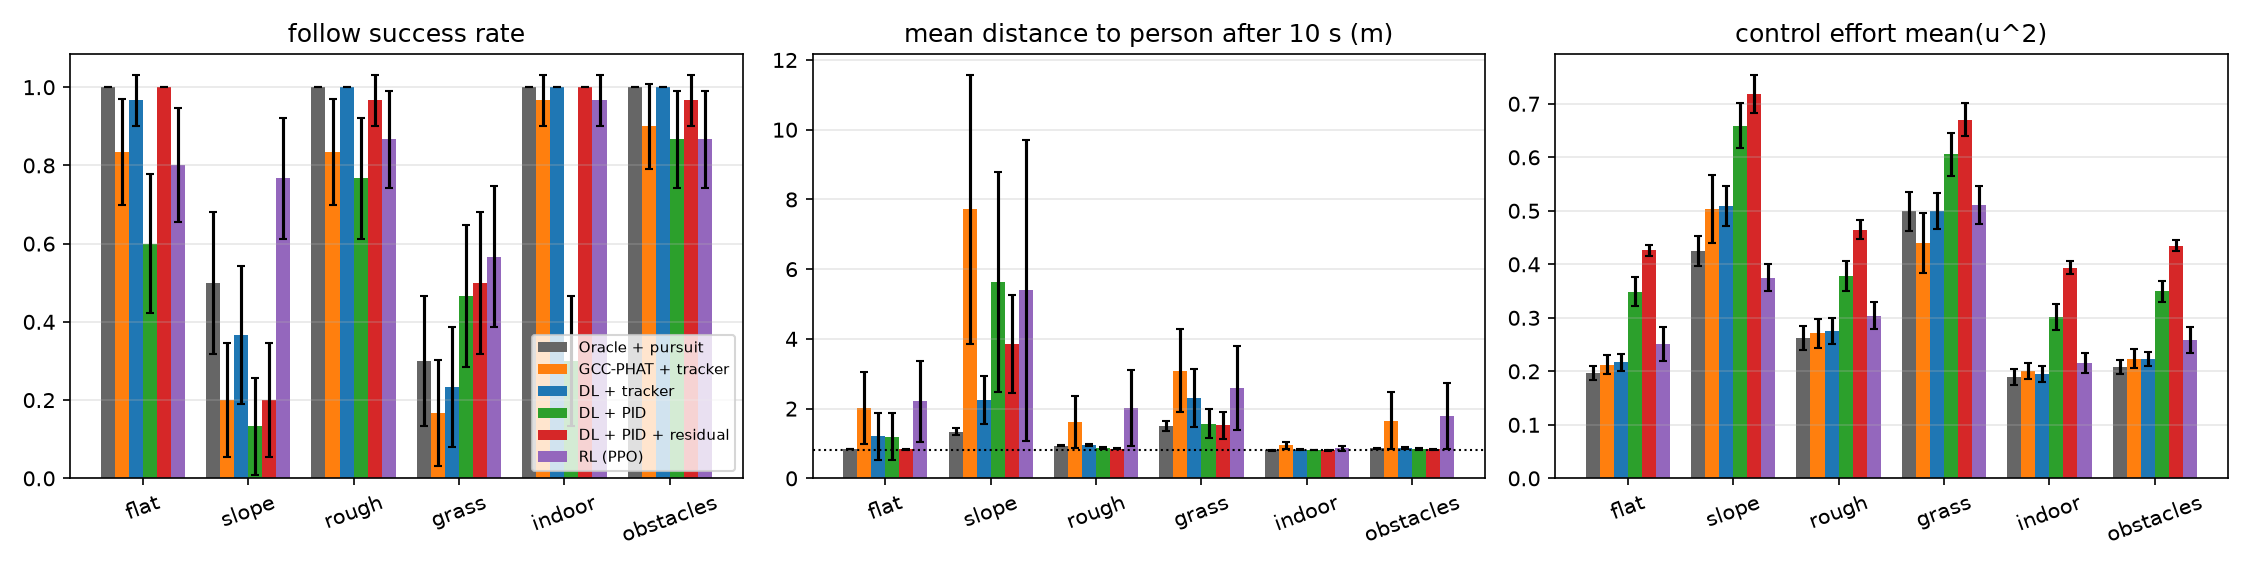
\includegraphics[width=\textwidth]{closed_loop_bars_B_fb.png}
\caption{Closed-loop results on channel B\_fb. Error bars: 95\% intervals over \CLBfbN{} episodes.}
\label{fig:bfbbars}
\end{figure*}

\section{Discussion}
\label{sec:discussion}

\textbf{What the deep localizer adds.} At this aperture and frequency the classical estimators
are not imprecise; their median errors are a few degrees. Their problem is a heavy tail of
wrong peaks: aliased lobes, reflections and noise when the direct path is weak. The deep model
inherits the steered response through its initialisation and learns which frames and which
lobes to trust. It halves the mean error and cuts range gross errors sharply, but it does not
remove the low-SNR tail (Fig.~\ref{fig:locsnr}). In closed loop the gain shows up as tighter
following on easy terrain, not as more successes.

\textbf{The comparison of controllers is confounded in two ways.} First, RL sees classical
acoustic features and the other learned controllers see the deep localizer, so RL's lead says
that a learned policy can compensate for poorer sensing with better driving, not that RL beats
deep localization. An RL policy on top of the deep localizer is the obvious next experiment,
and we did not run it. Second, our PID and pursuit gains were tuned by hand, and our PID lacks
a pitch limiter. A better-tuned classical controller would narrow the gap on slopes, but we have
not shown by how much. RL was trained on the simulator it is tested in, with randomised
terrain parameters but the same model. Against a real sphere it may lose more than the
model-based controllers, whose structure does not depend on the simulator.

\textbf{What the residual learned.} It learned how much duty, beyond what the flat-ground mixer
assumes, the current terrain needs to hold the current motion. It infers the terrain from the
last 0.5\,s of duties and proprioception and never sees a label. It helps where the inner loop
otherwise has to integrate a large load, and it smooths the cart's pitch. It does not make
slopes work: there the problem is the downhill drift and the cart's pitch limit, which no
feedforward on speed and yaw rate can fix.

\section{Limitations}

Everything is simulated. The acoustic model has no diffraction, no speaker directivity, no
body shadowing by the person carrying the phone, no wind, and no motor or rolling noise from
the robot itself, which would sit in the same band. The INMP441 response above 20\,kHz and the
decimation filter edges come from our model, not from measurement. Many phones do not emit
energy above 20\,kHz at all, which is why we report the fallback chirp, and that chirp is
audible to some people. Range depends on an emission schedule shared by phone and robot, which
we assume (100\,$\mu$s jitter, $\pm$200\,$\mu$s bias) but did not build. Without it only
bearing is available.

The sphere is modelled as planar pitch dynamics with a separate lateral pendulum and
first-order yaw, rolling without slip, and an inelastic wall contact. It is not a 3-D contact
model, and its parameters are not identified from a real robot. The simulator applies duties
up to 1.0 with no slew limit, while the firmware clamps to 0.8 and limits the slew to 4 per
second, so the deployed system is slower than the simulated one.

The residual network's design error was found with the oracle diagnostic, which runs on the
first \DbgN{} evaluation scenarios of four terrains (\DbgSeconds\,s each). Design decisions made
with this diagnostic, the residual fix in particular, were therefore not made on held-out
scenarios. The problem first showed up in the closed-loop evaluation itself: DL + PID + residual
succeeded in 2 of 30 flat episodes, with 16.6 tumble steps per episode
(\texttt{results/superseded\_closed\_loop\_A\_us\_run1.log}). We fixed the residual, discarded those rows and reran that controller on all
terrains. No other controller was changed after the evaluation started. The PPO run is a single seed. The localizer's best validation
epoch was its last, so it had not fully converged. Each closed-loop configuration was run once
with \CLAusN{} episodes. The 95\% intervals cover scenario variation, not training variation.

No result here is comparable to Daredevil \cite{constandache2014daredevil} or MilliSonic
\cite{wang2019millisonic}. Those systems were measured on hardware, with different signals,
geometries and goals.

\section{Conclusion}

In simulation, a localizer that starts from the SRP-PHAT steering of the actual array and
learns to weight frames halves the classical bearing MAE (\LocdlfullBMAE$^\circ$ against
\LocsrpphatBMAE$^\circ$) and cuts the range MAE from \LocsrpphatRMAE{} to \LocdlfullRMAE\,m on
the same \NTestSet{} test recordings. Phase is essential, since the magnitude-only model is at
chance. Multipath augmentation helps modestly. In closed loop, localization matters most on
easy terrain, while on slopes and grass the controller is the bottleneck: a PPO policy with
classical features was the most reliable follower (\CLAusrlsucc\% pooled success on the ideal
channel), and a learned terrain residual turned a tumbling cascaded PID into a reliable one on
flat, indoor and obstacle terrain. With a realistic front end and the 17--19.5\,kHz fallback
chirp, the deep localizer's closed-loop advantage grows (\CLBfbdltracksucc\% against
\CLBfbgcctracksucc\% success with the same tracker) and PPO's shrinks (\CLBfbrlsucc\%). The firmware and companion app implement the same command
protocol, but whether any of this holds on a real sphere with a real phone is untested.
